\chapter{Church-Turing Thesis}
\section{Turing Machines}
\begin{example}[Motivation for Turing Machines]
	Consider the language $\Ll = \{w\#w\mid w\in (0+1)^*\}$, this is not $\CFL$, in particular - not regular. With that said - given a word $00110\#00110$ (on the strip of a \TM), one can \textit{decide} if this word is in the language. This process can be described by a Turing machine:
	\begin{itemize}
		\item Check if the word is of the form $(0+1)^*\#(0+1)^*$. If not - \textit{reject}.
		\item Start from the first state, go to the symmetrical opposite, \textit{write} $X$ on the corresponding letters. If some corresponding pair do not agree - \textit{reject}.
	\end{itemize}
\end{example}
\begin{yellowBox}
	\begin{defn}
		[Deterministic Turing Machine] $\Mm = \tbk{Q,\Sigma, \Gamma, q_0, q_{acc}, q_{rej}, \delta}$ with:
		\begin{itemize}
			\item $Q$ finite set of configurations.
			\item $\Sigma$ alphabet, not containing \textbf{Blank Symbol} $\huge\textvisiblespace$.
			\item $\Gamma$ is \textbf{Working Alphabet} (\textbf{Tape} Alphabet) - the things the \TM can write on the strip. We demand $\Sigma\subset \Gamma$, and $\huge\textvisiblespace\in \Gamma$.
			\item $q_{0},q_{acc}\neq q_{rej}\in Q$ are start, accepting and rejecting states respectively.
			\item $\delta: Q\times \Gamma \to Q\times \Gamma \times \{L,R\}$. Meaning - when the machine is in state $q$ and the head is over a tape square containing a symbol $\gamma$, then $\delta(q,\gamma) = (q', \gamma', D)$ means that the machine overwrites $\gamma$ with $\gamma'$, goes to state $q'$ and moves over the tape in direction $D$.
		\end{itemize}
	\end{defn}
	\begin{remark}
		A DFA $\Aa$ is a specific instance of \TM, the intuition is $\delta(q,\sigma) = (q',\sigma, R)$. We will not get into this here.
	\end{remark}
	\begin{remark}
		Note the difference between state and block on strip.
	\end{remark}
	\begin{remark}
		The Nondeterministic setting is simply $\delta: Q\times \Gamma \to 2^{Q\times \Gamma \times \{L,R\}}$
	\end{remark}
\end{yellowBox}
\begin{yellowBox}
	\begin{defn}
		[Configurations] Let $\Mm$ be a \TM, the \textbf{Configuration} in which the current tape content is the words $uv$ (with $u,v\in \Gamma^*$), the head is over the first letter in $v$ and state $q$ - is denoted $uqv$. \\
		The collection of all configurations is $\Gamma^*Q\Gamma^*$, the \textbf{Initial} configuration is $q_0w$, an \textbf{Accepting/ Rejecting} configuration is one such that $q = q_{acc}, q_{rej}$ respectively. These two configurations are called \textbf{Halting} configurations.
	\end{defn}
	\begin{defn}
		[Yielding Configurations] Let $a,b\in \Gamma, u,v\in \Gamma^*, q\in Q$ and consider the configuration $uaqbv$ (that is, current state is $q$ and head over $b$ on the strip). If $\delta(q,b) = (q', c, L)$, then we say $uaqbv$ \textbf{Yields} the configuration $uq'acv$, denoted:
		\[
		uaqbv \To uq'acv
		\]
		We say that $uq'acv$ is consecutive (or subsequent) to $uaqbv$. \\
		Similarly, if $\delta(q,b) = (q', c, R)$, we say $uaqbv$ \textbf{Yields} the configuration $uacq'v$, denoted
		\[
		uaqbv \To uacq'v
		\]
		We say that $uacq'v$ is consecutive to $uaqbv$. \\
	\end{defn}
	\begin{defn}
		[Run of \TM on a word]
		Let $\Mm$ be a \TM. \textbf{The Run} on $\Mm$ on $w\in \Sigma^*$ is a sequence $\Rr = C_0, C_1\ldots $\footnote{Could be infinite!} such that $C_0$ is the initial configuration $C_0 = q_0w$ and for any $i\geq 1$, $C_{i+1}$ is \textbf{Yielded} by $C_i$, or that $C_i$ is a halting configuration.
	\end{defn}
	\begin{defn}[Accepting Run]
		We say the $w\in \Sigma^*$ is \textbf{accepted} by a \TM $\Mm$ if there exists a sequence of configurations $C_0\ldots C_m$\footnote{Note that $m$ could be even smaller than $|w|$} such that $C_0$ is the initial configuration of $\Mm$ on $w$ - $q_0w$, and for any $i<m$, $C_{i+1}$ is consecutive of $C_i$, and $C_m$ is accepting.
	\end{defn}
	\begin{defn}
		[Language of \TM, Recognize Language] We define the \textbf{Language of \TM} $\Mm$:\[
		\Ll(\Mm) = \{w\mid w\text{ is accepted by }\Mm\}
		\]
		We say that $\Mm$ \textbf{Recognizes} $\Ll$ if $\Ll(\Mm) = \Ll$. Alternatively - $\Ll$ is \textbf{Turing-recognizable}.
	\end{defn}
	\begin{defn}
		[Recursively Enumerable Languages, $\coRE$] We define $\RE$ to be the class of all languages recognized by some Turing machine. Define $\Ll\in \coRE \iff \Ll^c\in \RE$
	\end{defn}
\end{yellowBox}
Any \TM has three options on an input $w$: Halting (and rejecting\ accepting) or to not halt at all. An important note here is that for a recognizable language, we only demand halting on words that are in $\Ll$; for other words - $\Mm$ may not even halt. Therefore, we prefer Turing machines that halt on all inputs.

\begin{yellowBox}
	\begin{defn}
		[Decide a Language]We say $\Mm$ \textbf{Decides} a language $\Ll$ if $\Ll(\Mm) = \Ll$ and $\Mm$ halts on all inputs.
	\end{defn}
	\begin{defn}
		[Recursive languages] The class $\Rcr$ is the class of all Turing decidable languages.
	\end{defn}
	\begin{remark}
		It is clear that $\Rcr\subset \RE$, but we do not yet know if the containment is proper.
	\end{remark}
\end{yellowBox}
\begin{example}
	Consider the language $\Ll = \{w\#w\mid w\in (0+1)^*\}$. We want to show $\Ll\in \Rcr$.
	\begin{figure}[H]
		\centering
		\begin{tikzpicture}[every node/.style={block},
			block/.style={minimum height=1.7em,outer sep=0pt,draw,rectangle,node distance=0pt}]
			\node (A1) at (0,0) {$0$};
			\node (B1) [right=of A1] {$1$};
			\node (C1) [right=of B1] {$0$};
			\node (D1) [right=of C1] {$\small\#$};
			\node (E1) [right=of D1] {$0$};
			\node (F1) [right=of E1] {$0$};
			\node (G1) [right=of F1] {$1$};
			\node (H1) [right=of G1] {$\blank$};
			\node (head) [above = 0.5cm of A1,thick] {$q_0$};
			%			
			\draw[-latex,blue] ($(head.east)!0.5!(A1.east)$) -- ++(5mm,0);
			\draw[-latex] (head) -- (A1);
			\draw
			(H1.north east) -- ++(1cm,0) (H1.south east) -- ++ (1cm,0);
			
			\node (A2) at (0,-3) [text = red] {\textrm{X}};
			\node (B2) [right=of A2] {$1$};
			\node (C2) [right=of B2] {$0$};
			\node (D2) [right=of C2] {$\small\#$};
			\node (E2) [right=of D2] {$0$};
			\node (F2) [right=of E2] {$0$};
			\node (G2) [right=of F2] {$1$};
			\node (H2) [right=of G2] {$\blank$};
			\node (head2) [above = 0.5cm of E2,thick] {$q_1$};
			%			
			\draw[-latex,blue] ($(head2.west)!0.5!(E2.west)$) -- ++(-5mm,0);
			\draw[-latex] (head2) -- (E2);
			\draw
			(H2.north east) -- ++(1cm,0) (H2.south east) -- ++ (1cm,0);
			
			\node (A3) at (0,-6) {\textrm{X}};
			\node (B3) [right=of A3] {$1$};
			\node (C3) [right=of B3] {$0$};
			\node (D3) [right=of C3] {$\small\#$};
			\node (E3) [right=of D3, text = red] {\textrm{X}};
			\node (F3) [right=of E3] {$0$};
			\node (G3) [right=of F3] {$1$};
			\node (H3) [right=of G3] {$\blank$};
			\node (head3) [above = 0.5cm of A3,thick] {$q_2$};
			%			
			%				\draw[-latex,blue] ($(head2.west)!0.5!(E2.west)$) -- ++(-5mm,0);
			\draw[-latex] (head3) -- (A3);
			\draw
			(H3.north east) -- ++(1cm,0) (H3.south east) -- ++ (1cm,0);
			
			
			\node (A4) at (0,-9) {\textrm{X}};
			\node (B4) [right=of A4] {$1$};
			\node (C4) [right=of B4] {$0$};
			\node (D4) [right=of C4] {$\small\#$};
			\node (E4) [right=of D4] {\textrm{X}};
			\node (F4) [right=of E4] {$0$};
			\node (G4) [right=of F4] {$1$};
			\node (H4) [right=of G4] {$\blank$};
			\node (head4) [above = 0.5cm of B4,thick] {$q_3$};
			%			
			%				\draw[-latex,blue] ($(head2.west)!0.5!(E2.west)$) -- ++(-5mm,0);
			%				\draw[-latex] (head2) -- (E2);
			\draw[-latex] (head4) -- (B4);
			\draw
			(H4.north east) -- ++(1cm,0) (H4.south east) -- ++ (1cm,0);
			
			\node (A5) at (0,-12) {\textrm{X}};
			\node (B5) [right=of A5, text = red] {\textrm{X}};
			\node (C5) [right=of B5] {$0$};
			\node (D5) [right=of C5] {$\small\#$};
			\node (E5) [right=of D5] {\textrm{X}};
			\node (F5) [right=of E5] {$0$};
			\node (G5) [right=of F5] {$1$};
			\node (H5) [right=of G5] {$\blank$};
			\node (head5) [above = 0.5cm of F5,thick] {$q_4$};
			%			
			%				\draw[-latex,blue] ($(head2.west)!0.5!(E2.west)$) -- ++(-5mm,0);
			%				\draw[-latex] (head2) -- (E2);
			\draw[-latex] (head5) -- (F5);
			\draw
			(H5.north east) -- ++(1cm,0) (H5.south east) -- ++ (1cm,0);
			
			
		\end{tikzpicture}
		\caption{Example of the run on input $010\#001$ until transition to rejecting state}
	\end{figure}
	
	Idea:
	\begin{enumerate}
		\item Let the head be on the first block, if points on $\blank$ - reject.
		\item If the current block is not $\#$:
		\begin{enumerate}[2.1]
			\item Delete the current block, remember what was written.
			\item Move right until the last not-deleted character to the right of $\#$.
			\item If this character is different from what we remembered, or is $\#,\blank$ - reject. Else - delete it, and go left to the closest deleted character to $\#$, and move one block right. Return to $2$.
		\end{enumerate}
		\item Go right to the first not deleted character to the right on $\#$, if $\blank$ - accept. Else - reject.
	\end{enumerate}
	As a state machine, this looks like this:
	
	\begin{figure}[H]
		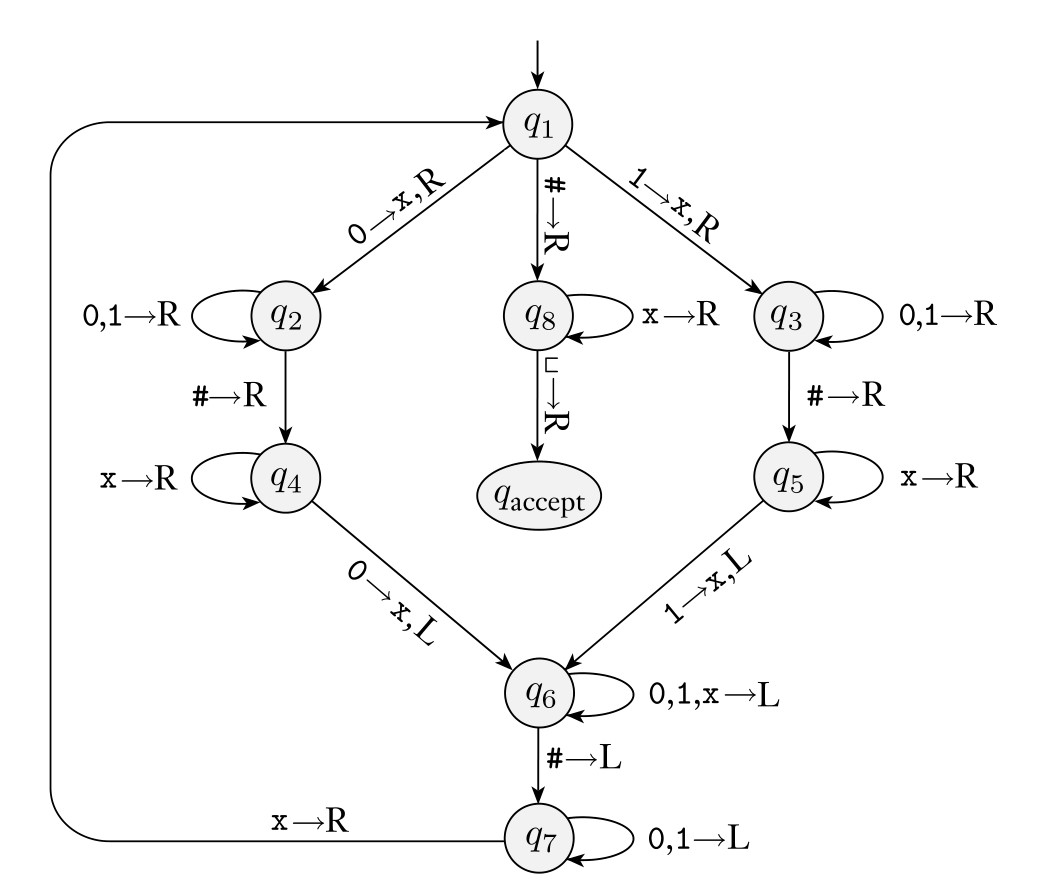
\includegraphics[scale=.5]{TMex1.jpg}
		\caption{Taken From the Book}
	\end{figure}
	
	%\begin{figure}[H]
	%	\centering
	%	\begin{tikzpicture}[shorten >=1pt,node distance=3cm,on grid,auto]
	%		\node[state,initial] (0)   {$q_0$};
	%		\node[state] (1) at (2,2) {$q_1$};
	%		\node[state] (2) at (2,-2) {$q_2$};
	%		\node[state] (3) at (4,2) {$q_3$};
	%		\node[state] (4) at (4,-2) {$q_4$};
	%		\node[state] (5) at (4,0) {$q_5$};
	%		\node[state] (6) at (2,0) {$q_6$};
	%		\node[state] (7) at (0,-2) {$q$};
	%		\node[state] (8) at (6,0) {$q_{acc}$};
	%		\node[state] (9) at (0,-4) {$q_{rej}$};
	%
	%		
	%		\path[-stealth, thick]
	%		(0) edge [bend left] node{$0\to X,R$} (1)
	%		edge [bend left] node{$1\to X,R$} (2)
	%		
	%		(1) edge [loop above] node{$0\to 0,R$ \\$1\to 1,R$} (1)
	%			;
	%	\end{tikzpicture}
	%	\caption{The visual representation of $\delta$ of the previous \TM description} \label{fig:M1}
	%\end{figure}
\end{example}
\begin{yellowBox}
	
	\begin{defn}
		[$\coRE$] Define the class:\[
		\coRE = \{\Ll\mid \Sigma^*\setminus \Ll = \Ll^c\in \RE\}
		\]
	\end{defn}
\end{yellowBox}


\subsection{Closure Properties of $\Rcr, \RE$}
\begin{blueBox}
	\begin{thm}
		$\Rcr$ is closed under complement.
	\end{thm}
\end{blueBox}
\begin{proof}
	Let $\Ll\in \Rcr$ and $\Mm$ \TM such that $\Ll(\Mm) = \Ll$. Define $\Mm'$ with $q_{qcc}' = q_{rej}$ and vice versa. Then still $\Mm'$ halts on any $w\in \Sigma^*$, and $w\in \Ll(\Mm')$ iff $w\notin \Ll(\Mm) = \Ll$ thus $\Ll(\Mm') = \Ll^c$.
\end{proof}
\begin{blueBox}
	\begin{thm}
		$\RE$ is closed under Union.
	\end{thm}
\end{blueBox}
\begin{proof}
	Let $\Ll_1,\Ll_2\in \RE$ and $\Mm_1,\Mm_2$ appropriate TMs. Define $\Mm$ the following way: First - move the input of the strip one place to the right, and add $\$$ at the start (can be done, see recitation), and add one more $\$$ at the end of the word. This one will never be deleted. Leave space for a counter, and add one more $\$$ and a bit indicating in which \TM we are at the moment, and one more $\$$. Afterwards - copy $w$ after the final $\$$. 
	
	\begin{figure}[H]
		\begin{tikzpicture}[every node/.style={block},
			block/.style={minimum height=1.5em,outer sep=0pt,draw,rectangle,node distance=0pt}]
			\node (A) {$\$$};
			\node (B) [right=of A] {$w$};
			\node (C) [right=of B] {$\$$};
			\node (D) [right=of C] {\textrm{counter}};
			\node (E) [right=of D] {$\$ $};
			\node (F) [right=of E] {\textrm{b}};
			\node (G) [right=of F] {$\$$};
			\node (H) [right=of G] {$w$};
			%  			\node (head) [above = 0.75cm of A,thick] {$q$};
			%			
			%			\draw[-latex,blue] ($(head.east)!0.5!(A.east)$) -- ++(5mm,0);
			%			\draw[-latex] (head) -- (A);
			\draw
			(H.north east) -- ++(1cm,0) (H.south east) -- ++ (1cm,0);
		\end{tikzpicture}
	\end{figure}
	$\Mm$ emulates the current machine's (according to the bit) run for $i$ (counter) steps. If the emulation accepts - accept the word. Otherwise - switch the bit. If $0\to 1$, increase $i ++$, check $w$ again using the other \TM.\\
	Let $w\in \Ll_1\cup \Ll_2$, then $\Mm_1$ (WLOG) accepts $w$ after $m$ steps, then when $\Mm$'s counter reaches $m$ - $\Mm$ accepts $w$, thus $w\in \Ll(\Mm)$. Conversely - if $w\in \Ll(\Mm)$, then $\Mm$ reached some accepting state in some emulation - hence $w\in \Ll_1\cup\Ll_2$.
\end{proof}

\subsection{Relationship between Turing classes}
\begin{blueBox}
	\begin{thm}
		\[
		\coRE \cap \RE = \Rcr
		\]
	\end{thm}
\end{blueBox}
\begin{proof}
	By definition - $\Rcr \subset \RE$. We show $\Rcr \subset \coRE$. Let $\Ll\in \Rcr$ and $\Mm_1$ a \TM deciding $\Ll$. Then $\widetilde{\Mm}_1$ defined by $\widetilde{q}_{acc} = q_{rej}$\footnote{Using the deterministic model. This in fact means that $\Rcr$ is closed under negation.} and vice versa, decides $\Ll^c$, hence $\Ll\in \coRE$, thus $\Rcr\subset \RE \cap \coRE$.\\
	Conversely - let $\Ll\in \RE\cap \coRE$, and $\Mm, \Mm^c$ TMs that recognize $\Ll,\Ll^c$ respectively. We build $\Mm$ that decides $\Ll$: Given $w\in \Sigma^*$, then $\Mm$ would operate in the following manner: 
	\begin{enumerate}
		\item Initialize a counter $i=0$.
		\item While we did not stop:\begin{enumerate}[2.1]
			\item $i += 1$
			\item Run $\Mm, \Mm^c$ on $w$ for $i$ steps. 
			\item If $\Mm$ accepted: Halt and accept.\footnote{Can reject if rejects}
			\item If $\Mm^c$ accepted: Halt and reject\footnote{Can accept if rejects}
		\end{enumerate}
	\end{enumerate}
	It is guaranteed $w\in \Ll \sqcup \Ll^c$, thus $\exists i$ s.t one of $\Mm, \Mm^c$ halts and accepts after $i$ steps - thus $\Mm$ always halts and either accepts or rejects and with the correct answer.
\end{proof}
\section{Variants of TMs}
\subsection{Enumerators}
An enumerator is a variant of Turing Machine - it is a \TM with a "printer": It has no input. It writes a sequence of words separated by $\#$ on the output strip. The language of an enumerator $\Ee$ is defined:\[
\Ll(\Ee) = \{w\mid \Ee\text{ prints }w\text{ at least once}\}\]
\begin{blueBox}
	\begin{thm}
		$\Ll\in \RE \iff$ there exists an enumerator $\Ee$ s.t $\Ll(\Ee) =\Ll$.
	\end{thm}
\end{blueBox}
\begin{proof}
	Let $\Ee$ be an enumerator with $\Ll(\Ee) = \Ll$. Define $\Mm$: given $w\in \Sigma^*$, $\Mm$ runs $\Ee$ and whenever $\Ee$ prints a new word $y$, $\Mm$ checks if $w = y$. If so - $\Mm$ halts and accepts. Correctness is obvious.\\
	Let $\Mm$ recognize $\Ll$, and build $\Ee$ s.t $\Ll(\Ee) = \Ee$. Let $\Tt$ be a lexicographic order of $\Sigma^*$\footnote{Countable!}. $\Ee$ would operate the following way:
	Initialize a counter $i$, run $\Mm$ on $w_1\ldots w_i$ for $i$ steps and print whenever $\Mm$ accepts $w_j$. Note that this always halts after at most $i^2$ steps. Afterwards - $i+=1$. Once again - correctness is obvious.
\end{proof}
\subsection{Nondeterminism}
\begin{yellowBox}
	\begin{defn}[nondeterministic TM]
		A \textbf{Nondeterministic TM} is defined in the expected way - by allowing "guesses". This is captured ny the fact that the transition function is:
		\[
		\delta:Q\times \Gamma \to 2^{Q\times \Gamma \times \{R,L\}}
		\]
	\end{defn}
	\begin{defn}[Decider]
		We say that a nondeterministic TM $\Mm$ is a \textbf{decider} if all computations of $\Mm$ halt.
	\end{defn}
\begin{defn}[Nondeterministic runtime]
	The runtime of a nondeterministic decider $\Mm$ on a word $w$ is the longest path in the run tree of $\Mm(w)$.
\end{defn}
\end{yellowBox}
\begin{example}
	Consider $\Cc = \{\tbk{n}\mid n\text{ is not a prime number}\}$. We build a nondeterministic TM that decides $\Cc$: Given $\tbk{n}$, guess a prime $p\leq n$ and check if it is a divisor of $n$. If so - accept, otherwise reject.
\end{example}
\begin{blueBox}
	\begin{thm}[Equivalence]
		For any nodeterministic decider $\Nn$ there exists a deterministic TM $\Mm$ with $\Ll(\Nn) = \Ll(\Mm)$.
\end{thm}\end{blueBox}
\begin{proof}
	The intuition here is using $BFS$ over the decision tree of $\Nn$: The root is the initial configuration and for any node, its children are all possible consecutive configurations. Define $\Mm$ the following way:\\
	Initialize an iteration. In the $i$th iteration - simulate $\Nn$'s run up to depth $i$ in it's run tree of $\Nn$ (this is the BFS idea). Note that the splitting degree of the tree is bounded by some constant $k$ - hence $BFS$ can be done. If at some point $\Nn$ accepts - accept, otherwise - reject (since $\Nn$ is a decider, this is well defined). Therefore
	\[
	\Mm(w) = acc \iff \text{There exists an accepting branch in $\Nn$'s run tree} \iff w\in \Ll(\Nn)
	\]
\end{proof}
What is the \textbf{cost} of translation? If $\Nn$ runs $t$ steps on $w$, then $\Mm$ runs $O(k^t\cdot t^2) = O(2^t)$ steps, with $k^t$ the maximal degree of a node in the run tree, and $t^2$ comes from BFS (number of edges).
\begin{blueBox}
	\begin{thm}[Characterization of 
		"nondeterministic languages"]
		Let $\Ll\subset \Sigma^*$. There exists a nondeterministic $\Nn$ with $\Ll = \Ll(\Nn)$ if and only if there exists $\Kk\in \Rcr$ such that \[
		\Ll = \{x\in \Sigma^*\mid \exists y\quad x\#y\in \Kk \}
		\]
		We should think of $y$ as a "witness" of $x\in \Ll$ - that is, $y$ is an "encoding of an accepting run of $\Nn$ over $x$.
	\end{thm}
\begin{remark}
	A machine $\Tt$ that decides $\Kk$ is called a \textbf{verifier} for $\Ll$.
\end{remark}
\end{blueBox}
\begin{proof}
	Let $\Nn$ be s.t $\Ll(\Nn) = \Ll$, and denote
	\[
	\Kk = \{x\#y\mid y\text{ describes an accepting run of $\Nn$ over $x$}\}
	\] Then if $x\in \Ll$ there exists an accepting run $y$ of $\Nn$ over $x$, hence $x\# y\in \Kk$. Conversely - if $x\#y\in \Kk$ then there exists an accepting run of $\Nn$ over $x$ (described by $y$) - so the construction is correct. It's left to show that $\Kk\in \Rcr$:
	Let $\Tt$ be a deterministic TM that receives $x\# y$ and checks that $y$ is a valid description of a run of $\Nn$ over $x$, and that the first configuration of $y$ corresponds to $q_{acc}^\Nn$, that all configurations are subsequent and if the last configuration is $q_{acc}^\Nn$. If so - accept. Otherwise, reject. Thus $\Kk\in \Rcr$.\\
	
	Conversely - Assume that there exists $\Kk\in \Rcr$ and $\Ll$ is of the ugly form. Construct $\Nn$ the following way: Guess all possible $\#y\in\Sigma^*_\Kk$. There are infinitely many possible $\# y$ - so the guess is done by sequentially guessing if adding another letter from $\Sigma_\Kk$ or to halt - this is of splitting degree $|\Sigma_\Kk| +1 $. After the guess - run $\Tt_\Kk$ over $x\# y$ (that is deterministic!). As for correctness - $x\in \Ll(\Nn)$ iff there is some $\# y$ such that $x \# y\in \Kk$. Note that $\Nn$ doesn't necessarily halt over all $x$.
\end{proof}

\begin{example}
	Consider $\Cc$ from earlier. Then $\Kk$ should be thought of as $x\# \tbk{p \text{ devisor}}$: $\Tt_\Kk$ over $x\#y$ will check $y\nim{?}\mid x$.
\end{example}

\section{The Definition of an Algorithm}
They developed the concept independently. Turing defined Turing Machine, and Church showed that $\lambda$-calculus is equivalent to \TM.\\
In 8.8.1900 - the best mathematicians met and described Hilbert's 23 problems. The 10'th problem was the following:
\begin{mdframed}
	\begin{center}
		\textit{Describe an algorithm that given a polynomial $p\in \ZZ[x_1\ldots x_k]$ - decide if there is an integer root $(n_1\ldots n_k)\in \ZZ^k$}
	\end{center}

\end{mdframed}
As for the definition of algorithm - Hilbert described an algorithm as "A process that can be decided after a finite number of steps". Today (1970), we know that there is no solution: This problem is not in $\Rcr$, thus this problem is undecidable. For our needs - an algorithm can be described in one of three levels:
\begin{enumerate}
	\item (Formal description) A Turing Machine $\Mm$
	\item (Implementation description) Description of operation of $\Mm$
	\item (High-Level description)Description by Pseudo-Code.
\end{enumerate}
We would like to be convinced that $2\iff 3$. There is a gap in \textbf{terminology}\footnote{Graphs, matrices, etc - compared to words.}. We will denote $\tbk{A}$ to describe an instance $A$. For example - describing Hilbert's problem as:
\[
D = \{\tbk{p}\mid p\text{ has an integer root}\}
\]
This is thinking of polynomials as words in some language, and a polynomial $6x^3yz^2+3xy^2-x^3-10$ is described on a strip as:
\begin{figure}[H]
	\begin{tikzpicture}[every node/.style={block},
		block/.style={minimum height=1.5em,outer sep=0pt,draw,rectangle,node distance=0pt}]
		\node (A) {$\$$};
		\node (B) [right=of A] {$6$};
		\node (C) [right=of B] {$x$};
		\node (D) [right=of C] {$3$};
		\node (E) [right=of D] {$y$};
		\node (F) [right=of E] {$z$};
		\node (G) [right=of F] {$2$};
		\node (H) [right=of G] {$+$};
		\node (I) [right=of H] {$3$};
		\node (J) [right=of I] {$x$};
		\node (K) [right=of J] {$y$};
		\node (L) [right=of K] {$2$};
		\node (M) [right=of L] {$-$};
		\node (N) [right=of M] {$x$};
		\node (O) [right=of N] {$3$};
		\node (P) [right=of O] {$-$};
		\node (Q) [right=of P] {$10$};
		\node (R) [right=of Q] {$\blank$};
		\node (S) [right=of R] {$\ldots$};
		%  			\node (head) [above = 0.75cm of A,thick] {$q$};
		%			
		%			\draw[-latex,blue] ($(head.east)!0.5!(A.east)$) -- ++(5mm,0);
		%			\draw[-latex] (head) -- (A);
		\draw
		(S.north east) -- ++(1cm,0) (S.south east) -- ++ (1cm,0);
	\end{tikzpicture}
\caption{Every number is encoded in binary, and we add some separators to avoid ambiguity}
\end{figure}
\begin{example}
	Describe a \TM for the problem of $G$ connectness. Formally:
	\[
	\Ll = \{\tbk{G}\mid G \text{ is an undirected connected graph}\}
	\]
	$G = (V,E)$ is encoded by enumerating the nodes $1\ldots n$ and writing them down in binary, separated by $\#$. When the nodes have ended - write $\$$ and start encoding the edges by pairs of nodes separated by $\#$ (or a new symbol, whatever)
	
	
	\begin{figure}[H]
		\begin{tikzpicture}[every node/.style={block},
			block/.style={minimum height=1.7em,outer sep=0pt,draw,rectangle,node distance=0pt}]
			\node (A) {$\$$};
			\node (B) [right=of A] {$0$};
			\node (C) [right=of B] {$0$};
			\node (D) [right=of C] {$\#$};
			\node (E) [right=of D] {$0$};
			\node (F) [right=of E] {$1$};
			\node (G) [right=of F] {$\#$};
			\node (H) [right=of G] {$1$};
			\node (I) [right=of H] {$0$};
			\node (J) [right=of I] {$\$$};
			\node (K) [right=of J] {$0$};
			\node (L) [right=of K] {$0$};
			\node (M) [right=of L] {$\#$};
			\node (N) [right=of M] {$0$};
			\node (O) [right=of N] {$1$};
			\node (P) [right=of O] {$\$$};
			\node (Q) [right=of P] {$0$};
			\node (R) [right=of Q] {$1$};
			\node (S) [right=of R] {$\#$};
			\node (T) [right=of S] {$\blank$};
			\node (U) [right=of T] {$\blank$};
			\node (V) [right=of U] {$\blank$};
			\node (W) [right=of V] {$\blank$};
			\node (X) [right=of W] {$\blank$};
			\node (Y) [right=of X] {$\blank$};
			\node (Z) [right=of Y] {$\ldots$};
			%  			\node (head) [above = 0.75cm of A,thick] {$q$};
			%			
			%			\draw[-latex,blue] ($(head.east)!0.5!(A.east)$) -- ++(5mm,0);
			%			\draw[-latex] (head) -- (A);
			\draw
			(Z.north east) -- ++(1cm,0) (Z.south east) -- ++ (1cm,0);
		\end{tikzpicture}
	\end{figure}
	Note that $\Ll^c = \{w\mid \text{does not describe a graph, or describes an unconnected graph}\}$. We will describe an algorithm to implement the algorithm:\\
	$\Gamma = \cbk{0,1,\#,\$,0_T,1_T, 0_A, 1_A, 0_C, 1_C}$ with the convention that a node with the first letter in its encoding is $0_T, 1_T$ is in $T$, $0_C,1_C$ in $C$ and $1_A,0_A$ is active (currently tested).
	\begin{enumerate}
		\item $T$-mark the first node.
		\item While there are $T$-marked nodes:
		\begin{enumerate}[2.1]
			\item $A$-mark a $T$-marked node.
			\item Scan the node list. If there is an unmarked node - check if there is an edge between it and the $A$-marked node. If so - $T$-mark it.
			\item $C$-mark the previously $A$-marked node.
		\end{enumerate}
		\item If all nodes are $C$-marked, accept. Else - reject.
	\end{enumerate}
	The goal here is to generally understand that Turing machines describe algorithms
	
\end{example}
\chapter{Decidability and Reducability}
In this chapter - we explore the question of decidability. Namely - what languages are decidable? Are there languages $\in \Rcr$ but not in $\RE$? How rich is $\RE$?\\
Let $\Sigma$ be a finite alphabet. Since there are $2^{\Sigma^*}$ languages, but all Turing machines are finite sequences - thus are countable. Since there is a surjective function $\TM\to \RE$, $\RE$ is countable. but $\RE\subset 2^{\Sigma^*}$ - so there must be at least one language with no \TM - hence $\RE$ is not everything.
\section{Undecidibility}
\begin{blueBox}
	\begin{thm}[Exsistance of undecidable langauges]
		\[\exists \Ll\notin \Rcr\]
		In particular - there exists a language $\Ll\notin \RE$ or $\Ll^c\notin \coRE$.
	\end{thm}
\end{blueBox}
\begin{proof}
	Consider the language $A_{\TM} = \cbk{\tbk{\Mm,w}\mid \Mm\text{ accepts }w}$. $A_{\TM}\in \RE$ for a \TM $\Hh$ that recognizes $A_{\TM}$, given $\tbk{\Mm,w}$ will run $\Mm$ on $w$.
	\begin{claim}
		$A_{\TM}\notin \Rcr$.
	\end{claim}
	By contradiction - let $\Hh$ be a \TM that decides $A_{\TM}$, that is:
	\[
	\Hh\left(\tbk{\Mm,w}\right) = \begin{cases}
		acc & \Mm(w) = acc\\
		rej & \Mm(w)\neq acc
	\end{cases}
	\]
	Note that the second cases encapsulates two options: either $\Mm(w)$ halts and rejects, or does not even stop! Now we build a new \TM $\Dd$ that gets an input $\tbk{\Mm}$ and operates the following way:
	\[
	\Dd(\tbk{\Mm}) = \begin{cases}
		acc & \Mm(\tbk{\Mm}) = acc\\
		rej & \Mm(\tbk{\Mm}) \neq acc
	\end{cases}
	\]
	Now, given $\Dd$ - build $\widetilde{\Dd}$ by flipping $q_{acc}$ and $q_{rej}$.\footnote{This is called \textbf{Diagonalization}.}\\
	Consider $\widetilde{\Dd}\left(\tbk{\widetilde{\Dd}}\right)$. That is:
	\[
	\widetilde{\Dd}\left(\tbk{\widetilde{\Dd}}\right) = \begin{cases}
		acc & \widetilde{\Dd}\left(\tbk{\widetilde{\Dd}}\right) \neq acc\\
		rej & \widetilde{\Dd}\left(\tbk{\widetilde{\Dd}}\right) = acc
	\end{cases}
	\]
	Which is a contradiction.	
\end{proof}
\subsection{The Halting Problem}
\begin{yellowBox}
	\begin{defn}
		Define $\HALT_{\TM} = \{\tbk{M,w}\mid M\text{ halts on }w\}$, that is - all Turing machines that halt on a word $w$.\\ Also define $\HALT_{\TM}^\varepsilon = \cbk{\tbk{\Mm}\mid \Mm(\varepsilon)\text{ halts}}$
	\end{defn}
\end{yellowBox}
\begin{blueBox}
	\begin{thm}
		$\HALT_{\TM}\notin \Rcr$
	\end{thm}
\end{blueBox}
\begin{proof}
	Let $\Mm'$ that decides $\HALT_{\TM}$, then if $\tbk{\Mm,w}\notin HALT$, then $\Mm$  doesn't halt on $w$, so $\tbk{\Mm,w}\notin A_{\TM}$, and the machine $\tbk{\Mm,w}$ decides $A_{\TM}$. Otherwise - if $\tbk{\Mm,w}\in \HALT_{\TM}$, then we can run $\Mm$ on $w$ and decide accordingly. That is - deciding $HALT$ means deciding $A_{\TM}$ - and as such,  $\HALT_{\TM}\notin \Rcr$
\end{proof}
This is called a proof by \textbf{Reduction}, 
\section{Reductions}
\begin{yellowBox}
	
	\begin{defn}[Computable Function]
		We say $f:\Sigma^* \to \Sigma^*$ is \textbf{Computable} if there exists $\Mm_f$ that on $w$ halts with $f(w)$ on the strip.
	\end{defn}
\end{yellowBox}
\begin{example}
	$f:\NN\times \NN \to \NN$ by $(x,y)\mapsto x+y$ by their unary representation.
	Then as input:
	\begin{figure}[H]
		\begin{tikzpicture}[every node/.style={block},
			block/.style={minimum height=1.7em,outer sep=0pt,draw,rectangle,node distance=0pt}]
			\node (A) {$1$};
			\node (B) [right=of A] {$1$};
			\node (C) [right=of B] {$1$};
			\node (D) [right=of C] {$1$};
			\node (E) [right=of D] {$\#$};
			\node (F) [right=of E] {$1$};
			\node (G) [right=of F] {$1$};
			\node (H) [right=of G] {$1$};
			\node (I) [right=of H] {$\blank$};
			\node (J) [right=of I] {$\blank$};
			\node (T) [right=of J] {$\blank$};
			\node (U) [right=of T] {$\blank$};
			\node (V) [right=of U] {$\blank$};
			\node (W) [right=of V] {$\blank$};
			\node (X) [right=of W] {$\blank$};
			\node (Y) [right=of X] {$\blank$};
			\node (Z) [right=of Y] {$\ldots$};
			%  			\node (head) [above = 0.75cm of A,thick] {$q$};
			%			
			%			\draw[-latex,blue] ($(head.east)!0.5!(A.east)$) -- ++(5mm,0);
			%			\draw[-latex] (head) -- (A);
			\draw
			(Z.north east) -- ++(1cm,0) (Z.south east) -- ++ (1cm,0);
		\end{tikzpicture}
	\end{figure}
	and as output
	\begin{figure}[H]
		\begin{tikzpicture}[every node/.style={block},
			block/.style={minimum height=1.7em,outer sep=0pt,draw,rectangle,node distance=0pt}]
			\node (A) {$1$};
			\node (B) [right=of A] {$1$};
			\node (C) [right=of B] {$1$};
			\node (D) [right=of C] {$1$};
			\node (E) [right=of D] {$1$};
			\node (F) [right=of E] {$1$};
			\node (G) [right=of F] {$1$};
			\node (H) [right=of G] {$\blank$};
			\node (I) [right=of H] {$\blank$};
			\node (J) [right=of I] {$\blank$};
			\node (T) [right=of J] {$\blank$};
			\node (U) [right=of T] {$\blank$};
			\node (V) [right=of U] {$\blank$};
			\node (W) [right=of V] {$\blank$};
			\node (X) [right=of W] {$\blank$};
			\node (Y) [right=of X] {$\blank$};
			\node (Z) [right=of Y] {$\ldots$};
			%  			\node (head) [above = 0.75cm of A,thick] {$q$};
			%			
			%			\draw[-latex,blue] ($(head.east)!0.5!(A.east)$) -- ++(5mm,0);
			%			\draw[-latex] (head) -- (A);
			\draw
			(Z.north east) -- ++(1cm,0) (Z.south east) -- ++ (1cm,0);
		\end{tikzpicture}
	\end{figure}
	
\end{example}
\begin{example}
	A function $f:\TM \to \TM$ such that $f(\Mm)$ is a \TM that does not halt on $w\notin \Ll(\Mm)$. That is - the machine $f(\Mm)$ loops whenever $\Mm$ rejects. THis is computable - we'll add a state $q_{loop}$ and transitions that were suppose to end with $q_{rej}$ will now go to $q_{loop}$, and of course a loop $q_{loop}\to q_{loop}$. Correctness is obvious.
\end{example}
\begin{example}
	[Uncomputable function - $BB$] Let $\Gamma = \cbk{0,1\blank}$. Define $BB$\footnote{Busy Beaver} by
	\[
	BB(k) = \text{The maximal number of $1$'s written on the strip of a TM with $k$ states over $\Gamma$ that halt over $\varepsilon$}
	\]
	\begin{prop}[1]
		$BB(k)$ is strictly increasing.
	\end{prop}
\begin{proof}
	Let $k\in \NN$ and $\Mm$ that achieve the maximum (that is - $\Mm$ of $k$ states and there are $BB(k)$ ones after $\Mm(\varepsilon)$ halts). Construct $\Mm'$ by switching $q^\Mm_{acc}$ by a new state that searches for a blank space on the strips and writes down $1$ (then moves to an accepting state). Thus $BB(k+1)\geq BB(k) + 1 > BB(k)$.
\end{proof}
\begin{prop}[2]
	$BB$ is not computable. That is, $BB\notin \Rcr$.
\end{prop}
\begin{proof}
	By contradiction - let $\Hh$ be a TM that computes $BB$, and assume $\Hh$ has $n$ states. WLOG $\Hh$ accepts as input and outputs numbers in binary representation. First - construct $\Mm_n$ with $\lceil\log(n)\rceil +1 $ states that halts over $\varepsilon$ and returns the binary representation of $2n$. Define a TM $\Mm$ that given $\varepsilon$, run $\Mm_n$ and then run $\Hh$ (over $2n$ in binary representation - now written on the strip). That is - $\Mm$ computes $BB(2n)$. Now - $\Mm$ has $n + \lceil\log(n)\rceil + 1$ states, and computes $BB(2n)$ - but $2n > n + \lceil\log(n)\rceil + 1$. This means that $\Mm$ shows that $BB(2n)\leq BB(n + \lceil\log(n)\rceil + 1)$ - which is a contradiction to proposition (1).\end{proof}
\end{example}
\begin{yellowBox}
	\begin{defn}[Mapping Reducable]
		We say that $A\subset \Sigma^*$ is \textbf{Mapping Reducable} to $B\subset\Sigma^*$ if there exists a computable function $f:\Sigma^* \to \Sigma^*$ such that $w\in A\iff f(w)\in B$. The function $f$ is called \textbf{Reduction} from $A$ to $B$. \\
		It is common to denote $A\leq_{m}B$.
	\end{defn}
\end{yellowBox}
\begin{remark}
	This allows us to translate membership questions.
\end{remark}
\begin{example}
	Consider $A = \{x\mid |x|\leq 5\}, B = \{x\mid |x|\leq 10\}$ over $\ZZ$. Note that the identity function is \emph{not} a reduction. $f(x) = 2x$ is a reduction.
\end{example}
\begin{blueBox}
	\begin{thm}["Reduction theorem"]
		If $A$ is reducable to $B$, then $B\in \Rcr \Rightarrow A\in \Rcr$.
	\end{thm}
\begin{remark}
	It is better to think of the theorem in the counter-positive description.
\end{remark}
\end{blueBox}
\begin{proof}
	Let $B\in \Rcr$, and let $\Mm_B,f$ be a \TM and a reduction from $A$ to $B$. Define $\Mm_A$ by the following procedure, given $w$:
	\begin{enumerate}
		\item Compute $M_{f(w)}$
		\item Run $\Mm_B(f(w))$.
	\end{enumerate}
	It is guaranteed that $\Mm_B$ accepts $M_{f(w)}$ iff $f(w)\in B$ iff $w\in A$, and $\Mm_A$ halts since $\Mm_f, \Mm_B$ halts.
\end{proof}
\begin{remark}
	We will use this theorem mostly to show Undecidability. As usual - use the counter-positive of the theorem: $A\leq_m B$ and $A\notin \Rcr$, then $B\notin \Rcr$.
\end{remark}
\begin{blueBox}
	\begin{thm}[More variations on Reduction theorem] Let $\Ll_1,\Ll_2$ languages over $\Sigma$.
	\begin{enumerate}
		\item $\Ll_2\in \RE \Longrightarrow \Ll_1\in \RE$
		\item $\Ll_2\in \coRE \Longrightarrow \Ll_1\in \coRE$
	\end{enumerate}
\end{thm}
\end{blueBox}
\begin{proof}
	[Proof (of 2.):]
	Let $\Ll_1\notin \coRE$, and $f:\Sigma^* \to \Sigma^*$ a reduction $\Ll_1\leq_m \Ll_2$, that is $f(x)\in \Ll_2 \iff x\in \Ll_1$. Notice that $f$ is therefore a reduction $\Ll_1^c \leq_m \Ll_2^c$. That is - $\Ll_1^c\notin \RE$ implies $\Ll_2^c\notin \RE$, hence $\Ll_2\notin\coRE$.
\end{proof}
\begin{example}
	(Another way to show the same thing) Consider $\HALT_{\TM}$, we want to show $A_{\TM}\leq_m \HALT_{\TM}$, thus $\HALT_{\TM}\notin \Rcr$. \\
	Consider the function $f:\tbk{\Mm,w}\mapsto\tbk{\Mm',w'}$ Given $\tbk{\Mm,w}$, create (the machine $\Mm_f$ will create) $\tbk{\Mm',w'}$ such that $\tbk{\Mm,w}\in A_{\TM} \iff \tbk{\Mm',w'}\in \HALT_{\TM}$. Consider the same function from before - $f$ would be the function that transforms $\Mm$ into $\Mm'$ that halts only if a word is accepted. Note that indeed - if $\tbk{\Mm,w}\in A_{\TM}$, and as such $\tbk{\Mm',w'}\in \HALT_{\TM}$. If $\tbk{\Mm,w}\notin A_{\TM}$ then $\Mm$ doesn't accept $w$, as such - $\Mm'$ doesn't halt on $w$, so $\tbk{\Mm',w'}\notin \HALT_{\TM}$, since we are not guaranteed that $\Mm'$ halts. Hence $f$ is a reduction, thus $\HALT_{\TM}\notin \Rcr$.
\end{example}
\begin{example}
	Consider $\HALT_{\TM}^\varepsilon \in \RE$, and $f:\HALT_{\TM}\to \HALT_{\TM}^\varepsilon$ defined by \[
	\tbk{\Mm,w}\nim{f}\mapsto \Mm_w \quad \Mm_w\text{ Moves the reading head to the left, write $w$ on the strip and runs $\Mm$ on $w$}
	\]
	Of course $\Mm(w)$ halts iff $\Mm_w$ halts on $\varepsilon$, thus $f$ is a mapping reduction from $\HALT_{\TM}^\varepsilon$ to $\HALT_{\TM}$, thus $\HALT_{\TM}^\varepsilon\notin \Rcr$.\\
	
	Note that $g:\HALT_{\TM}^\varepsilon \to \HALT_{\TM}$ by $\tbk{\Mm}\nim{g}\mapsto\tbk{\Mm,\varepsilon}$ is a reduction.
\end{example}
\begin{example}[More sophisticated]
	Consider the language $\Reg_{\TM}$ of all \TM such that $\Ll(\Mm)\in \Reg$. We show $\Reg_{\TM}\notin \Rcr$. We show a reduction $A_{\TM}\leq_m \Reg_{\TM}$:
	\[
	f:A_{\TM}\to \Reg_{\TM}\quad \tbk{\Mm,w}\mapsto \tbk{\Mm'}
	\]
	$\Mm'$ operates over $x\in \{0,1\}^*$ the following way:\\
	If $x\in \{0^n1^n\}$ then $\Mm'(x) = acc$, otherwise - $\Mm'$ runs $\Mm$ on $w$ and behaves the same way. Note that the computation of $f(\tbk{\Mm,w})$ is within finite time. We show $\tbk{\Mm,w}\in A_\TM \iff \Mm'\in \Reg_{\TM}$:\\
	If $\Mm(w) = acc$, then $\Ll(\Mm') = (0+1)^*\in \Reg$, thus $\tbk{\Mm'}\in \Reg_{\TM}$. If $\Mm(w) = rej$, then $\Ll(\Mm') = \{0^n1^n\}\notin \Reg$, thus $\tbk{\Mm'}\notin \Reg_{\TM}$ - hence $f$ is indeed a reduction $\Reg_{\TM}\to A_\TM$.
\end{example}
\begin{example}
	Let $\ALL_\TM = \cbk{\tbk{\Mm}\mid \Ll(\Mm) = \Sigma^*}$, we show that $\ALL_\TM\notin \RE\cup \coRE$:\\
	We show $\ALL_\TM\notin \coRE$ by reduction from $A_\TM$ to $\ALL_\TM$: We want a function $\tbk{\Mm,w}\nim{f}\mapsto \Mm'$ with $\Mm(w) = acc$ iff $\Ll(\Mm') = \Sigma^*$. Define $\Mm'$ to operate the following way: On input $x$, accept iff $\Mm(w)$ accepts, that is $\Mm'(x) = \Mm(w)$ for any $x\in \Sigma^*$. Note that $\Ll(\Mm') = \Sigma^*$ iff $\Mm'$ accepts all $x$ iff $\Mm(w) = acc$, that is $f$ is indeed a mapping reduction $A_\TM\leq_m \ALL_\TM$. Since $A_\TM\notin \coRE$, so is $\ALL_\TM$.\\
	Now, we show $\ALL_\TM\notin \RE$. We know that $A_\TM^c\notin \RE$, hence define
	\[
	f:A_\TM^c\to \ALL_\TM \quad \tbk{\Mm,w}\mapsto \Tt_{\Mm,w} = \Tt
	\]
	Given $x$, $\Tt$ would emulate $\Mm(w)$ for $|x|$ steps, and reject iff $\Mm$ accepted $w$. If $\tbk{\Mm,w}\notin A_\TM$, then $\Mm(w) \neq acc$, then $\Tt$ would accept any word $x$, hence $\Ll(\Tt) = \Sigma^*$. Otherwise - for a large enough $x$, $\Tt(x) = rej$, hence $\Ll(\Tt)\neq \Sigma^*$. Therefore $A_\TM^c\leq_m \ALL_\TM$. Since $A_\TM^c\notin \RE$, so is $\ALL_\TM$.
\end{example}
\begin{mdframed}
	There are many more examples in Recitation 7 notes - one should go over them. Reductions are difficult and are learned by examples and exercises.
\end{mdframed}
\subsection*{Then Tiling Problem}
The Tiling problem is an algorithmic problem. The input is a finite set $T$ of tiles with an initial tile $t_{init}$. Any tile is a square (triangalized) with different colors, and a legal tiling is such that two tiles are possible neighbors if the colors match. Formally - there are horizontal relations $H\subset T\times T$ and vertical relations $V\subset T\times T$. A legal $n\times n$ tiling is a function $f:[n]\times [n]\to T$ such that:
\begin{itemize}
	\item $f(1,1) = t_{init}$
	\item For any $i,j$: $H\left(f(i,j), f(i+1,j)\right)$ and $V\left(f(i,j), f(i,j+1)\right)$
\end{itemize}
\subsubsection*{Formalizing with our tools}
Let $TILE = \cbk{\tbk{T,H,V,t_{init}}\mid \text{There is a legal tiling for all }n}$. We would like to decide where does $TILE$ reside in the language classes. 
\begin{prop}
	$TILE\in \coRE$.
\end{prop}
\begin{proof}
	Consider $T$ that recognizes $TILE^c$:
	\begin{enumerate}
		\item Initialize $i = 1$
		\item Check all tilings of $[i]\times [i]$.
		\begin{itemize}
			\item If found a legal tiling - $i+=1$.
			\item If no legal tiling - accept.
		\end{itemize}
	\end{enumerate}
\end{proof}
\begin{prop}
	$TILE\notin \RE$. 
\end{prop}
\begin{proof}
	Surprisingly - we reduce $(HALT_\TM^\varepsilon)^c$ to $TILE$. The intuition is that an infinite run of $\Mm$ on $\varepsilon$ corresponds to a tiling of $\NN\times \NN$. 
	\begin{claim}
		There is a legal tiling for all $n$ $\iff$ there is a legal tiling of $\NN\times \NN$.
	\end{claim}
	\begin{proof}[Proof (of the claim)]
			$\Leftarrow$ is easy. We prove $\Rightarrow$. Recall Kőnig's lemma\footnote{In an infinite tree with a finite degree for any node there is an infinite path.}. We construct a tree with $i^{th}$ level nodes corresponding to $[i]\times [i]$ tilings, and an edge between a subtiling $f_{i-1}\subset f_i$. This tree is indeed connected and acyclic \footnote{Add explanation}. Thus there is an infinite path - corresponding to a tiling of $\NN\times \NN$.
	\end{proof}
We now construct the reduction. The idea - every floor in the tiling is a configuration, and transition between floors correspond to transition between subsequent configuration. We need to define $T$ so that an infinite tiling corresponds to a run:
\begin{itemize}
	\item The tiles in the first row:
	\begin{figure}[H]
		\begin{subfigure}{.5\textwidth}
			\centering
			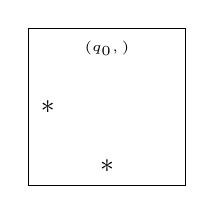
\begin{tikzpicture}
				\draw (-1,-1) -- (-1,1) -- (1,1) -- (1,-1) -- (-1,-1);
				\node at (0,.75) {\tiny$(q_0,\blank)$};
				\node at (.75, 0 ){\tiny$\blank$};
				\node at (0,-.75 ){$*$};
				\node at (-.75, 0 ){$*$};
			\end{tikzpicture}
		\caption{Initial tile}
		\end{subfigure}
	\begin{subfigure}{.5\textwidth}
					\centering
		\begin{tikzpicture}
			\draw (-1,-1) -- (-1,1) -- (1,1) -- (1,-1) -- (-1,-1);
			\node at (0,.75) {\tiny$\blank$};
			\node at (.75, 0 ){\tiny$\blank$};
			\node at (0,-.75 ){$*$};
			\node at (-.75, 0 ){\tiny$\blank$};
		\end{tikzpicture}
	\end{subfigure}
	\end{figure}
\item Tiles for simulating $R$ movement: For any transition $\delta(q,a) = (q', b, R)$ for $q\neq q_{acc}, q_{rej}$ we add $|\Gamma| + 1$ tiles
	\begin{figure}[H]
\begin{subfigure}{.5\textwidth}
			\centering
		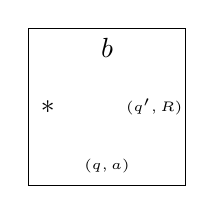
\begin{tikzpicture}
			\draw (-1,-1) -- (-1,1) -- (1,1) -- (1,-1) -- (-1,-1);
			\node at (0,.75) {$b$}; % Top
			\node at (.6, 0 ){\tiny$(q',R)$}; % right
			\node at (0,-.75 ){\tiny$(q,a)$}; %bottom
			\node at (-.75, 0 ){$*$}; %right
		\end{tikzpicture}
\end{subfigure}	
\begin{subfigure}{.5\textwidth}
	\centering
	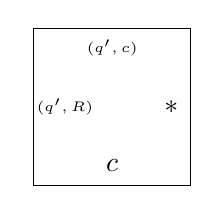
\begin{tikzpicture}
		\draw (-1,-1) -- (-1,1) -- (1,1) -- (1,-1) -- (-1,-1);
		\node at (0,.75) {\tiny$(q',c)$}; % Top
		\node at (-.6, 0 ){\tiny$(q',R)$}; % left
		\node at (0,-.75 ){$c$}; %bottom
		\node at (.75, 0 ){$*$}; %right
	\end{tikzpicture}
	\caption{for all $c\in \Gamma$}
\end{subfigure}	
\end{figure}
\item Tiles for simulating $L$ movement: For any transition $\delta(q,a) = (q', b, L)$ for $q\neq q_{acc}, q_{rej}$ we add $|\Gamma| + 1$ tiles
\begin{figure}[H]
	\begin{subfigure}{.5\textwidth}
		\centering
		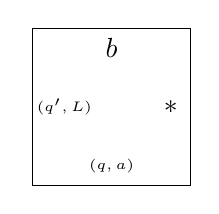
\begin{tikzpicture}
			\draw (-1,-1) -- (-1,1) -- (1,1) -- (1,-1) -- (-1,-1);
			\node at (0,.75) {$b$}; % Top
			\node at (-.6, 0 ){\tiny$(q',L)$}; % right
			\node at (0,-.75 ){\tiny$(q,a)$}; %bottom
			\node at (.75, 0 ){$*$}; %right
		\end{tikzpicture}
	\end{subfigure}	
	\begin{subfigure}{.5\textwidth}
		\centering
		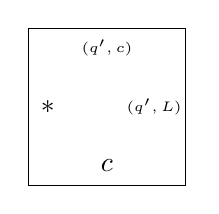
\begin{tikzpicture}
			\draw (-1,-1) -- (-1,1) -- (1,1) -- (1,-1) -- (-1,-1);
			\node at (0,.75) {\tiny$(q',c)$}; % Top
			\node at (.6, 0 ){\tiny$(q',L)$}; % right
			\node at (0,-.75 ){$c$}; %bottom
			\node at (-.75, 0 ){$*$}; %left
		\end{tikzpicture}
		\caption{for all $c\in \Gamma$}
	\end{subfigure}	
\end{figure}
\item Padding:
\begin{figure}[H]
	\centering
	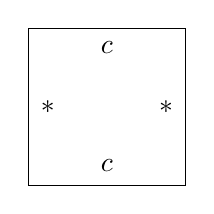
\begin{tikzpicture}
		\draw (-1,-1) -- (-1,1) -- (1,1) -- (1,-1) -- (-1,-1);
		\node at (0,.75) {$c$}; % Top
		\node at (.75, 0 ){$*$}; % right
		\node at (0,-.75 ){$c$}; %bottom
		\node at (-.75, 0 ){$*$}; %left
	\end{tikzpicture}
	\caption{for all $c\in \Gamma$}
\end{figure}
\end{itemize}
Note that this defines a mapping from TMs $\tbk{\Mm}$ into legal encodings of $TILE$. It is left to show that this is computable and that the reduction is correct:\\
For computability - given an encoding of $\delta$, there are finitely many tiles to encode - so this is computable.\\
For correctness - there exists an infinite tiling of our construction iff there is an inifnite sequence of configurations $C_0\ldots$ such that $C_i$ is written in the transition from row $i$ to row $i+1$, iff $C_0$ an initial configuration of $\Mm$ over $\varepsilon$ and $C_{i+1}$ is subsequent to $C_i$ iff $\Mm(\varepsilon)$ doesn't halt.
\end{proof}
